\documentclass{chi2009}
\usepackage{times}
\usepackage{url}
\usepackage{graphics}
\usepackage{color}
\usepackage[pdftex]{hyperref}
\hypersetup{%
pdftitle={Web-based Data Analytics in Haskell},
pdfauthor={Drew Haven, Eric Stratmann},
pdfkeywords={haskell, analytics},
bookmarksnumbered,
pdfstartview={FitH},
colorlinks,
citecolor=black,
filecolor=black,
linkcolor=black,
urlcolor=black,
breaklinks=true,
}
\newcommand{\comment}[1]{}
\definecolor{Orange}{rgb}{1,0.5,0}
\newcommand{\todo}[1]{\textsf{\textbf{\textcolor{Orange}{[[#1]]}}}}

\pagenumbering{arabic}  % Arabic page numbers for submission.  Remove this line to eliminate page numbers for the camera ready copy

\begin{document}
% to make various LaTeX processors do the right thing with page size
\special{papersize=8.5in,11in}
\setlength{\paperheight}{11in}
\setlength{\paperwidth}{8.5in}
\setlength{\pdfpageheight}{\paperheight}
\setlength{\pdfpagewidth}{\paperwidth}

% use this command to override the default ACM copyright statement 
% (e.g. for preprints). Remove for camera ready copy.
\toappear{CS240 Class Project}

\title{FOOBAR: Web-based Data Analytics in Haskell}
\numberofauthors{2}
\author{
  \alignauthor Drew Haven\\
    \affaddr{Stanford University}\\
    \email{drew.haven@gmail.com}
  \alignauthor Eric Stratmann\\
    \affaddr{Stanford University}\\
    \email{eric.stratmann@gmail.com}
}

\maketitle

\begin{abstract}
Many people are interested in statistics, but providing an easy to use Website to analyze statistics can be difficult. We wanted to make it simple to create Websites to analyze arbitrary data, so we created a Haskell package that makes it easy to do this. We also wrote an example site using our package that analyzes data from the popular on-line game League of Legends. The Website allows users to lookup a variety of statistics and perform queries on the data.
\end{abstract}

\section{Introduction}

Analyzing statistics can be rewarding and insightful, but without an easy way to analyze new datasets doing so can be difficult. Statistics are useful in a verity of fields. For example, although no knowledge of statistics is required to play baseball, many fans of the sport love to analyze them. Since baseball is popular there are many Websites to analyze baseball data, but what about less popular data? Creating a site to analyze new sets of data can be time consuming.

Although the data being analyzed across different datasets may differ considerably, the sorts of queries that people are interseted in are often similar. People would like to correlate different variables, filter on certain conditions, and retrieve subsets of the data. They would like to do calculations on the data (sums, averages, counts) and display this information in tables or charts. 

We have created FOOBAR~\cite{foobar}, a data analytics package written in Haskell that makes it convenient to write Websites to analyze arbitrary data. Our package allows developers to easily create a Website that allows users to query data from any dataset of their choosing and do other neat things. Since it is written in Haskell, our package takes advantage of Haskell features such as type safety. 

We created  a demo application using data from the on-line video game, League of Legends~\cite{lol}. League of Legends is a competitive Real Time Strategy games where teams of players compete against each other. The site allows users to view player information, analyze different variables, and other neat stuff. Users can analyze their own data to learn about their behavior in the game or look at more general data to see trends in gameplay. 

Todo: References don't work.
The rest of the paper is organized as follows. Section \ref{background} provides some background. We discuss our package in section \ref{package}. Section \ref{site} looks at our example site. In section \ref{future} we discuss possible future directions of our work. We provide an analysis of our results in section \ref{analysis}. Finally, section \ref{conflusion} concludes.

\section{Background, Technologies Used, Related Work, etc.}
\label{sec:background}

\subsection{Yesod}

Yesod~\cite{yesod} is one of several Web frameworks written in Haskell. Features of Yesod include templates, a persistence model, etc. Writing a Website in a Haskell framework allows developers to take advantage of Haskell features, such as type safety, which helps them write secure sites.

Yesod's type safety allows X. This can prevent XSS attacks. Prevents bad URLs (tells you when they're broken at compile time).

\begin{figure}[]
\begin{verbatim}
getGameIndexR :: Handler RepHtml
getGameIndexR = do
  (games, opts) <- paginateSelectList 10 [] []
  defaultLayout $ do
    let list = $(widgetFile "game/list")
    setTitle "Game Index"
    toWidget [cassius|
      ##header {
        float: left;
        color = #{color}}
    |] 
    $(widgetFile "game/index")
\end{verbatim}
    \caption{Sample Yesod Controller}
    \label{controller}
\end{figure}

\begin{figure}[]
\begin{verbatim}
^{pager opts}

<table.game-list>
<thead>
  <tr>
    <th>
      Teams
    <th>
      Queue
    <th>
      Date Added
<tbody>
  $forall game <- games
    <tr data-href=@{GameViewR (fst game)}>
      <td.champs>
        ^{portraits champions (snd game)}
      <td.queueType>
        #{gsqueueType (gameGameStats (snd game))}
      <td.created>
        #{gameFormattedCreateTime (snd game)}
\end{verbatim}
    \caption{Sample Hamlet File}
    \label{hamlet}
\end{figure}

\subsection{MongoDB}

Our backend used MongoDB~\cite{mongo}, a documented-oriented database. MongoDB stores data in BSON, a data format similar to JSON. MongoDB allows the execution of Javascript queries against the database. Although MongoDB is schemaless, you can use Haskell's type safety to ensure that only valid data is stored. We chose MongoDB becuase of X.

\subsection{Flot}

To generate charts, we use Flot~\cite{flot}, a Javascript charting library. We originally used the Chart package, but switched to Flot for compatability reasons and because Javascript charts are more dynamic. Since Flot did not have Haskell bindings, we had to write our own. 

\subsection{League of Legends}

League of Legends~\cite{lol} in an on-line Real Time Strategy game. Although the details are not important since we have chosen any other dataset to analyze, we provide a quick introduction of the important concepts to put the examples into context. Players (also known as summoners) fight on teams against each other using characters known as Champions. The object of the game is to advance on the other side's base. Players can advance towards this objective by killing other players and doing other stuff. People are interested in different statistics of summoners and champions, such as their kill and death rates. 

\subsection{Analytics packages}

There are lots of existing software that does similiar stuff. Here are a few of them. 

\section{Description of our project}
\label{package}

\subsection{Data backend}

Data is stored in mongodb and represented like X.

We use Yesod's Perist model which allows us to run queries from Yesod.

By usign type families and Haskell's type safety, we can ensure that only valid data is stored in the database. 

Talk about the Query API

Queries generate javascript code which is executed by mongo.

Generate mapreduce queries. See figure \ref{mrapi}.

\begin{figure*}[t]
\begin{verbatim}
type Game = GameGeneric backend
type GameId = Key backend Game
GameCreated :: EntityField Game UTCTime
GameGameStats :: EntityField Game GameStats

selectList :: (PersistEntity val, PersistBackend b m) => [Filter val] ->
              [SelectOpt val] -> b m [(Key b val, val)]
selectList [GameCreated <. time] [LimitTo 10] :: PersistBackend b m => b m [(GameId, Game)]
\end{verbatim}
    \caption{Query stuff}
    \label{querycode}
\end{figure*}

\begin{figure*}[t]
\begin{verbatim}
mapReduce :: (PersistBackend Action m, Applicative m, Queryable model)
  => QueryColumn model typ                 -- ^ The column to use a key.
  -> [QueryFilter model]                   -- ^ A list of filters.
  -> forall typ0. [QueryColumn model typ0] -- ^ A list of columns to select for the output.
  -> Action m [(Label, M.Map Label Value)]
\end{verbatim}
    \caption{MapReduce API}
    \label{mrapi}
\end{figure*}

\subsection{Chart generation}

FOOBAR displays appropriate information using Javascript charts. While some data is best presented in tabular form, charts can visually display the relationship of different variables in a way that is easy for people to understand.

We use the Flot Javascript charting package. Flot charts are generated using Javascript and displayed on an HTML Canvas element. 

While it is possible for developers to manually generate Javascript to create Flot charts, we created a Haskell API that allows developers to specify their charts in Haskell. The API seperates display options of the chart from the chart data.

Figure \ref{chartcode} shows a page that uses the chart API. The code creates a chart with the given options and uses the data retrieved from the query. The chart automatically takes care of including any necessary HTML, Javascript, and CSS and can simply be included anywhere in the page. Figure \ref{chart} shows a sample chart that shows information about X.

\begin{figure}[]
\begin{verbatim}
getFooR :: Handler RepHtml
getFooR = do
    data <- runDB blah buildQuery blah
        (QuerySomething foo) []
        [Query Something])
    let chart = myChart data
    ...

myChart :: Widget
myChart = 
    setTitles "XAxis" "YAxis" "Title" $
    setHorizontal True $
    setSize 600 400 $
    barChart
\end{verbatim}
    \caption{Chart API}
    \label{chartcode}
\end{figure}

\begin{figure}[h]
    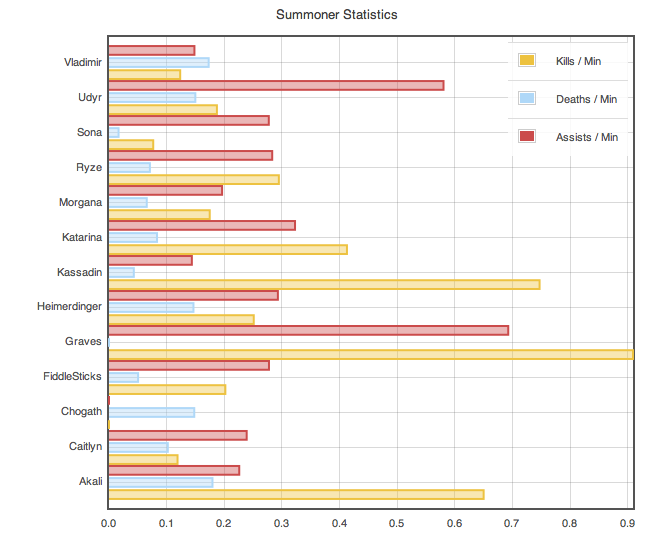
\includegraphics[width=80mm]{imgs/chart.png}
    \caption{Chart}
    \label{chart}
\end{figure}

\subsection{League of Legends Logs}

\begin{figure}[]
\begin{verbatim}
parseActionScript :: Parser ByteString ASValue
\end{verbatim}
    \caption{ActionScript parser API}
    \label{asapi}
\end{figure}

Data is parsed from LoL data files. Our parser uses attoparsec.

Figure \ref{asapi} shows the API.

\subsection{League of Legends Client}

Then it is uploaded using our client which monitors the file system for log files, parses them, and uploads them to the website. 

\section{League of Legends Site}
\label{site}

To test our data analytics package, we wrote a Website to display League of Legends statistics.

On the Websites, users can do X, Y, and Z. 

The site provides a variety of statistics on different summoners. Users can view statistics by different champions for any summoners, either in table or chart form. This allows users to do things like check correlations between different variables. 

In Figure \ref{chart}, we can see a chart (replace with more up to date chart). The chart shows some statistics for Summoner Foo. 

In Figure \ref{list}, we can see a list of games. Probably want a more interesting picture though.

\begin{figure}[h]
    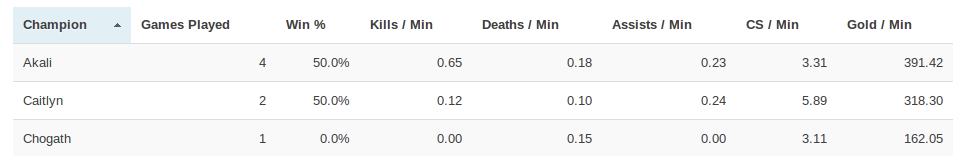
\includegraphics[width=80mm]{imgs/stats.png}
    \caption{Statistics for a summoner}
    \label{chart}
\end{figure}

\begin{figure}[h]
    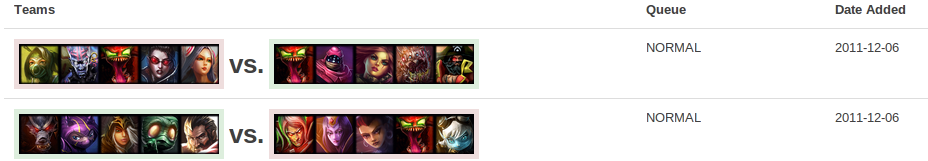
\includegraphics[width=80mm]{imgs/gamelist.png}
    \caption{Game list}
    \label{list}
\end{figure}

\section{Future Work}
\label{future}

What would be needed to bring this site to a production level?

* More work!

* Static file handling.  Yesod is not optimized for it.

* Load balancing and clustering.

* User accouts/permissions.  Fortunately most of this work has already been done.

\section{Analysis}
\label{analysis}

We learned X.

Features X, Y, and Z of Haskell/Yesod/etc. were lacking and we'd like to see some improvements.

Features X, Y, and Z of Haskell/Yesod/etc. were great and gave us the following benefits.

Overall we were pleased/displeased/had no strong feelings about our project.

\section{Conclusion}
\label{conclusion}

Data analytics can be fun and exciting. We created a Website to analyze League of Legends data, but can be used with a variety of data.

Our project shows that Haskell is a good/ok/bad language for data analytics, although X. 

\bibliographystyle{abbrv}
\bibliography{paper}

\end{document}
